\documentclass[]{report}
\usepackage{graphicx, float,}
\usepackage{hyperref}
\usepackage[export]{adjustbox}

\title{\centering CSD300 : Design Project \\Music Genre Recognition}
\author{\LARGE Vaibhav Vashisht\\ \LARGE 2016UCS0002\\ \\ \LARGE Sahil\\ \LARGE 2016UCS0008}

% to use proper section numbering in the report type 
\renewcommand{\thesection}{\arabic{section}}

\begin{document} 

\maketitle

%%%%%%%%%%%%%%%%%%%%%%%%%%%%%%%%%%%%%%%%%%%%%%%%
\section{Problem Statement:}
\large 
\begin{itemize}
	\item Wikipedia defines music genre as a conventional category that identifies pieces of music as belonging to a shared tradition or set of conventions.
	\item Classifying songs according to genre is something that has been till now done by human tagging. The necessity for such a tagged dataset arises for any music search engine that aims to suggest similar songs to the user.
	\item Characteristics that define a song to be in a particular genre are usually somewhat abstract and often a song may have overlapping genres. 
	\item To automate the task of genre classification one first needs a suitable feature vector to represent the song. We aim to classify genre independent of the metadata (artist information, lyrics etc).
\end{itemize}  

\section{Methodology:}
\large 
Here’s a general overview of what we will do:
\begin{itemize}
	\item Extract a simplified representation of the songs (.wav file).
	\\
	In brief, the song will be converted to a spectrogram which is a visual representation of the spectrum of frequencies of sound as they vary with time. A mel spectrogram will be suitable for this purpose. 

	\item Train a neural network to classify the songs. 
	\begin{itemize}
	\item As we are treating our music file as a spectrogram, in other words our input is an image hence we can use CNN to train our Deep Learning model. 
	\item But, since music genre is based on the combination of small pieces of a musical track which are dependent on each other, hence the genre of our audio file will depend on the relation between each small portion, hence using sequential deep learning models may give better results.
	\item So, to overcome this difficulty, a convolutional recurrent neural network involving CNN and LSTM can be used. The resulting sequence of features created from a CNN layer, can be fed to a LSTM layer, which will find both dependencies across short period of time, and a long term structure of the song. 
	\end{itemize}
	\item Use the classifier to find the genre.
	\\
	The output from previous layers can then be fed to fully connected layer with softmax activation, giving 10-D vectors for each timestamp.
	\\ 
	We can take mean across the time dimension to get the most likely genre of the song.
	
	
\end{itemize}

\begin{figure}[H]
	\vspace{0pt}
	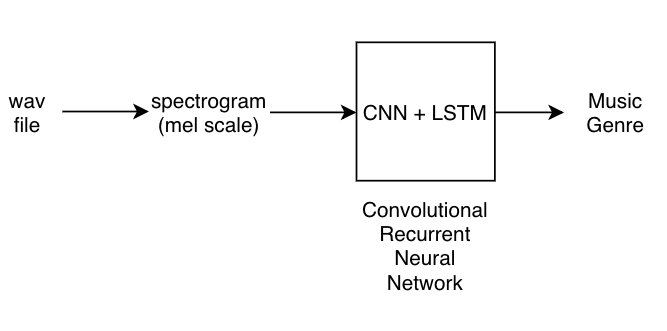
\includegraphics[height = 150pt, keepaspectratio]{methodology.png}
\end{figure}

\section{Tools/softwares required:}
\begin{itemize}
	\item \textbf{Librosa:} is a python package for music and audio analysis.
	\item \textbf{PyTorch or Keras:} for neural networks. 
	\item \textbf{Google Colab:} for training the model on GPU (if required).
	
\end{itemize}
\section{Data collection:}
\begin{itemize}
	\item The \textbf{GTZAN} dataset, used for the well known paper in genre classification "Musical
	genre classification of audio signals" by G. Tzanetakis and P. Cook in IEEE
	Transactions on Audio and Speech Processing 2002 is considered.
	\item The dataset consists of 1000 audio tracks each 30 seconds long. 
	\item It contains 10 genres, each represented by 100 tracks.
	\item The tracks are all 22050Hz Mono 16-bit audio files in .wav format.
\end{itemize}

\section{References}
The following article has been used as a reference: \url{http://deepsound.io/music_genre_recognition.html}.
\end{document}